% ===================================
% CODICE LaTeX PER GRAFICI E TABELLE
% Tesi GDO - Capitoli 1 e 2
% ===================================
% filepath: c:\Users\saint\tesi\nuovi grafi 1 e 2.tex
\documentclass[varwidth=true,border=10pt]{standalone}
% Pacchetti necessari
\usepackage[utf8]{inputenc}
\usepackage[T1]{fontenc}
\usepackage{amsmath}
\usepackage{amssymb}    
\usepackage{graphicx}
\usepackage{caption}
\usepackage{subcaption} % Per sottotitoli nelle figure
% Preambolo necessario:
\usepackage{tikz}
\usepackage{pgfplots}
\usepackage{booktabs}
\usepackage{multirow}
\pgfplotsset{compat=1.17}
\usetikzlibrary{pgfplots.polar}
% FIGURA 1.3: Decomposizione del Framework GIST
\begin{document}
\begin{figure}[h]
\centering
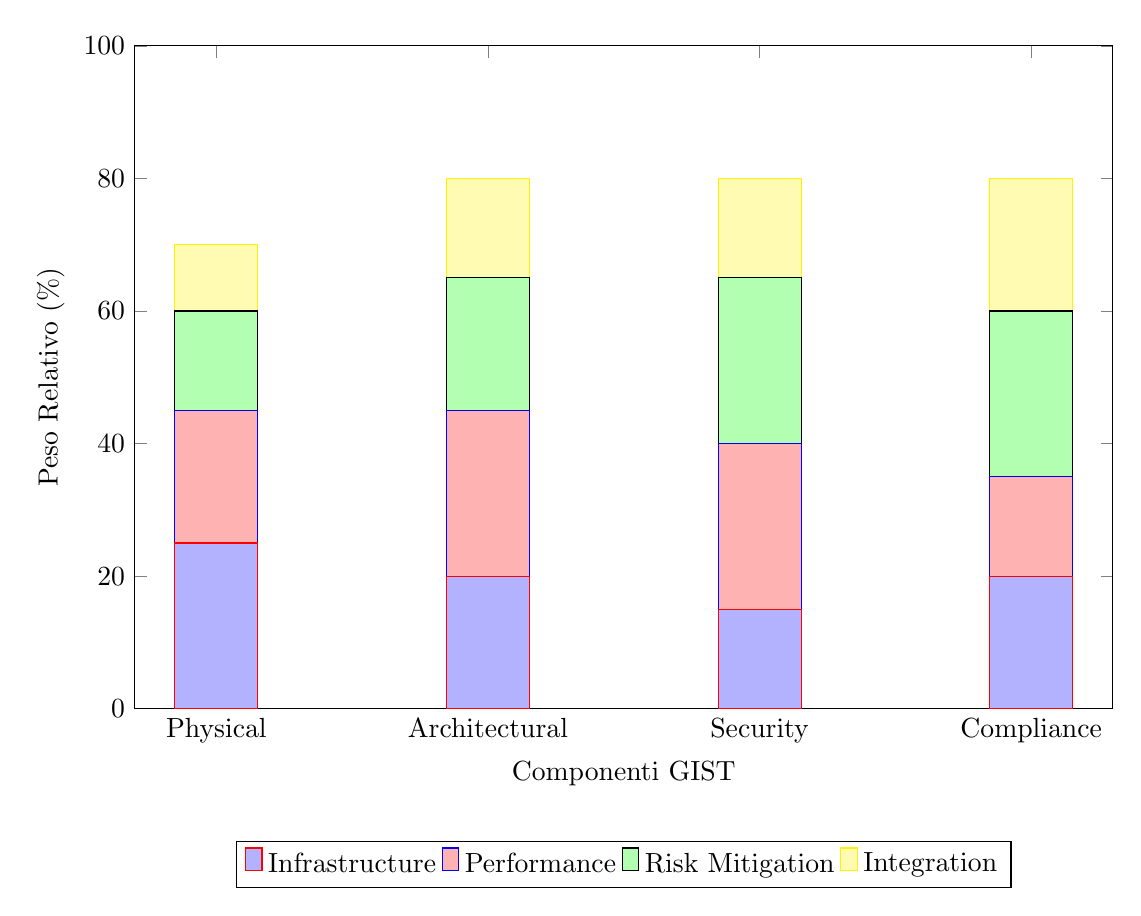
\begin{tikzpicture}
\begin{axis}[
    width=14cm,
    height=10cm,
    ybar stacked,
    ylabel={Peso Relativo (\%)},
    xlabel={Componenti GIST},
    symbolic x coords={Physical,Architectural,Security,Compliance},
    xtick=data,
    ymin=0,
    ymax=100,
    bar width=30pt,
    legend style={at={(0.5,-0.2)},anchor=north,legend columns=4},
    cycle list name=color list
]
\addplot+[ybar,fill=blue!30] coordinates {(Physical,25) (Architectural,20) (Security,15) (Compliance,20)};
\addplot+[ybar,fill=red!30] coordinates {(Physical,20) (Architectural,25) (Security,25) (Compliance,15)};
\addplot+[ybar,fill=green!30] coordinates {(Physical,15) (Architectural,20) (Security,25) (Compliance,25)};
\addplot+[ybar,fill=yellow!30] coordinates {(Physical,10) (Architectural,15) (Security,15) (Compliance,20)};

\legend{Infrastructure,Performance,Risk Mitigation,Integration}
\end{axis}
\end{tikzpicture}
\caption{Decomposizione dei pesi relativi nel Framework GIST per diversi scenari operativi}
\label{fig:gist_decomposition}
\end{figure}
\end{document}